%% RiSE Latex Template - version 0.5
%%
%% RiSE's latex template for thesis and dissertations
%% http://risetemplate.sourceforge.net
%%
%% (c) 2012 Yguaratã Cerqueira Cavalcanti (yguarata@gmail.com)
%%          Vinicius Cardoso Garcia (vinicius.garcia@gmail.com)
%%
%% This document was initially based on UFPEThesis template, from Paulo Gustavo
%% S. Fonseca.
%%
%% ACKNOWLEDGEMENTS
%%
%% We would like to thanks the RiSE's researchers community, the 
%% students from Federal University of Pernambuco, and other users that have
%% been contributing to this projects with comments and patches.
%%
%% GENERAL INSTRUCTIONS
%%
%% We strongly recommend you to compile your documents using pdflatex command.
%% It is also recommend use the texlipse plugin for Eclipse to edit your documents.
%%
%% Options for \documentclass command:
%%         * Idiom
%%           pt   - Portguese (default)
%%           en   - English
%%
%%         * Text type
%%           bsc  - B.Sc. Thesis
%%           msc  - M.Sc. Thesis (default)
%%           qual - PHD qualification (not tested yet)
%%           prop - PHD proposal (not tested yet)
%%           phd  - PHD thesis
%%
%%         * Media
%%           scr  - to eletronic version (PDF) / see the users guide
%%
%%         * Pagination
%%           oneside - unique face press
%%           twoside - two faces press
%%
%%		   * Line spacing
%%           singlespacing  - the same as using \linespread{1}
%%           onehalfspacing - the same as using \linespread{1.3}
%%           doublespacing  - the same as using \linespread{1.6}
%%
%% Reference commands. Use the following commands to make references in your
%% text:
%%          \figref  -- for Figure reference
%%          \tabref  -- for Table reference
%%          \eqnref  -- for equation reference
%%          \chapref -- for chapter reference
%%          \secref  -- for section reference
%%          \appref  -- for appendix reference
%%          \axiref  -- for axiom reference
%%          \conjref -- for conjecture reference
%%          \defref  -- for definition reference
%%          \lemref  -- for lemma reference
%%          \theoref -- for theorem reference
%%          \corref  -- for corollary reference
%%          \propref -- for proprosition reference
%%          \pgref   -- for page reference
%%
%%          Example: See \chapref{chap:introduction}. It will produce 
%%                   'See Chapter 1', in case of English language.

\documentclass[en,twoside,onehalfspacing,phd]{risethesis}

\usepackage[english]{babel}
\usepackage{colortbl}
\usepackage{color}
\usepackage[table]{xcolor}
\usepackage{microtype}
\usepackage{bibentry}
\usepackage{subfigure}
\usepackage{multirow}
\usepackage{rotating}
\usepackage{booktabs}
\usepackage{pdfpages}
\usepackage{caption}
\usepackage{lipsum}

\captionsetup[table]{position=top,justification=centering,width=.85\textwidth,labelfont=bf,font=small}
\captionsetup[lstlisting]{position=top,justification=centering,width=.85\textwidth,labelfont=bf,font=small}
\captionsetup[figure]{position=bottom,justification=centering,width=.85\textwidth,labelfont=bf,font=small}

%% Remove colors from hyperlinks
\makeatletter
\AtBeginDocument{%
  \renewcommand*{\AC@hyperlink}[2]{%
    \begingroup
      \hypersetup{hidelinks}%
      \hyperlink{#1}{#2}%
    \endgroup
  }%
}
\makeatother

%% Change the following pdf author attribute name to your name.
\usepackage[linkcolor=black,
            citecolor=blue,
            urlcolor=black,
            colorlinks,
            pdfpagelabels,
            pdftitle={Rise Thesis Template (ABNT)},
            pdfauthor={Rise Thesis Template (ABNT)}]{hyperref}

\address{RECIFE}

\universitypt{Universidade Federal de Pernambuco}
\universityen{Federal University of Pernambuco}

\departmentpt{Centro de Informática}
\departmenten{Center for Informatics}

\programpt{Pós-graduação em Ciência da Computação}
\programen{Graduate in Computer Science}

\majorfieldpt{Ciência da Computação}
\majorfielden{Computer Science}

\title{An Automated Approach to Assign Software Change Requests}

\date{2014}

\author{Yguaratã Cerqueira Cavalcanti}
\adviser{Silvio Romero de Lemos Meira}
\coadviser{Eduardo Santana de Almeida}

% Macros (defines your own macros here, if needed)
\def\x{\checkmark}

\begin{document}

\frontmatter

\frontpage

\presentationpage

\begin{fichacatalografica}
	\FakeFichaCatalografica % Comment this line when you have the correct file
%     \includepdf{fig_ficha_catalografica.pdf} % Uncomment this
\end{fichacatalografica}

\banca

\begin{dedicatory}
I dedicate this thesis to all my family, friends and professors who gave me the
necessary support to get here.
\end{dedicatory}

\acknowledgements
\lipsum[1-4]

\begin{epigraph}[]{Poul Anderson}
I have yet to see any problem, however complicated, which, when looked at in the
right way, did not become still more complicated.
\end{epigraph}

\resumo
% Escreva seu resumo no arquivo resumo.tex
O gerenciamento eficiente de solicitações de mudança (SM) é fundamental para o
sucesso das atividades de manutenção e evolução de software. Entretanto, a
atribuição de SMs a desenvolvedores de software é um aspecto custoso desse
gerenciamento, pois demanda tempo e requer conhecimento apropriado do projeto de
software. Com o propósito de diminuir esse custo, várias pesquisas já propuseram
métodos de atribuição automática de SMs. Embora representem avanços na área,
existem vários fatores inerentes a atribuição de SMs que não são considerados
nessas pesquisas e são essenciais para a automação.

Como demonstrado nesse trabalho, a atribuição automática deve, por exemplo,
considerar a carga de trabalho, a experiência e o conhecimento dos
desenvolvedores, a prioridade e a severidade das SMs, a afinidade dos
desenvolvedores com os problemas descritos nas SMs, e até mesmo os
relacionamentos interpessoais. Para tornar esse cenário ainda mais complexo,
esses fatos podem variar de acordo com o projeto de software que está sendo
desenvolvido. Assim, uma solução para o problema de atribuição de SMs depende de
informações contextuais.

Assim, esse trabalho propõe, implementa e valida uma solução arquitetural
sensível ao contexto para atribuição automática de SMs. Dado o aspecto
contextual da solução, a arquitetura enfatiza a necessidade de considerar as
diversas fontes de informações presentes na organização, assim como a
necessidade de se desenvolver algorítimos que implementem diferentes estratégias
de atribuição. A proposta e implementação dessa solução é embasada em resultados
de duas pesquisas quantitativas: um estudo de mapeamento sistemático da
literatura, e uma pesquisa de questionário com desenvolvedores de software. Esse
último forneceu um conjunto de requisitos que a solução automatizada deve
satisfazer para que as estratégias de atribuição sejam atendidas, enquanto o
mapeamento da literatura identificou técnicas, algoritmos, e outros requisitos
necessários a automação.

A implementação da arquitetura segue uma estratégia de automação, também
elabo\-rada nesse trabalho, que possui dois componentes principais: um sistema
especialista baseado em regras (SEBR); e um modelo de recuperação de informação
(MRI) com técnicas de aprendizagem. Em nossa estratégia, esses dois componentes
são executados alternadamente em momentos diferentes a fim de atribuir uma SM
automaticamente. O SEBR processa regras simples e complexas, considerando
informações contextuais do projeto de software e da organização que o
desenvolve. O MRI é utilizado para fazer o casamento entre SMs e desenvolvedores
de acordo com o histórico de atribuições.

\begin{keywords}
Engenharia de Software, Manutenção e Evolução de Software, Gerenciamento de
Solicitações de Mudança, Atribuição Automática de Solicitações de Mudança
\end{keywords}

\abstract
% Write your abstract in a file called abstract.tex
Software maintenance and evolution are characterised by their huge cost and
slow speed of implementation. Yet they are inevitable activities -- almost all
software that is useful and successful stimulates user-generated requests for
change and improvements. \citeauthor{Sommerville2007} is
even more emphatic and says that software changes is a fact of life for large
software systems. In addition, a set of studies has stated along the years that
software maintenance and evolution is the most expensive phase of software
development, taking up to 90\% of the total costs.

All those characteristics from software maintenance lead the academia and
industry to constantly investigate new solutions to reduce costs in such
phase. In this context, Software Configuration Management (SCM) is a set of
activities and standards for managing and evolving software; SCM defines how
to record and process proposed system changes, how to relate these to system
components, among other procedures. For all these tasks it has been proposed
different tools, such as version control systems and bug trackers. However, some
issues may arise due to these tools usage, such as the dynamic assignment of a
developer to a bug report or the bug report duplication problem.

In this sense, this dissertation investigates the problem of bug report
duplication emerged by the use of bug trackers on software development
projects. The problem of bug report duplication is characterized by the
submission of two or more bug reports that describe the same software issue, and
the main consequence of this problem is the overhead of rework when managing
these bug reports.

\begin{keywords}
bug reports, bug trackers, bug report duplication, change request,
tool experiment, bug report duplication characterization study, bug report
search and analysis tool
\end{keywords}

% List of figures
\listoffigures

% List of tables
\listoftables

% List of acronyms
% Acronyms manual: http://linorg.usp.br/CTAN/macros/latex/contrib/acronym/acronym.pdf
\listofacronyms
\chapter*{List of Acronyms}
\addcontentsline{toc}{chapter}{List of Acronyms}
\begin{acronym}[C.E.S.A.R.]
  \acro{AJAX}{Asynchronous JavaScript and XML}
  \acro{BAST}{Bug Report Analysis and Search Tool}
  \acro{BTT}{Bug Report Tracker Tool}
  \acro{BRN}{Bug Report Network}
  \acro{CCB}{Change Control Board}
  \acro{C.E.S.A.R.}{Recife Center For Advanced Studies and Systems
  \acroextra{C.E.S.A.R. (\url{http://www.cesar.org.br}) is a CMMi level 3
  company with around 700 employees}}
  \acro{FR}{Functional Requirement}
  \acro{GQM}{Goal Question Metric}
  \acro{LOC}{Lines of Code}
  \acro{NFR}{Non-Functional Requirement}
  \acro{NLP}{Natural Language Processing}
  \acro{ORM}{Object-Relational Mapper}
  \acro{RiSE}{Reuse in Software Engineering Group \acroextra{\url{http://www.rise.com.br}}}
  \acro{SCM}{Software Configuration Management}
  \acro{SD}{Standard Deviation}
  \acro{TF-IDF}{Term Frequency-Inverse Document Frequency}
  \acro{UFPE}{Federal University of Pernambuco}
  \acro{VSM}{Vector Space Model}
  \acro{WAD}{Work as Design}
  \acro{XP}{eXtreme Programming}
\end{acronym}

% Summary (tables of contents)
\tableofcontents

\mainmatter

\chapter{Introduction}
\label{chp:introduction}

% \begin{quotation}[]{Poul Anderson}
% I have yet to see any problem, however complicated, which, when looked at in the
% right way, did not become still more complicated.
% \end{quotation}

Software maintenance starts as early as the first software artifacts are
delivered, and is characterized by its high cost and slow speed of
implementation~\citep{swebok2004}. It has been stated that it is the most
expensive activity of software development, taking up to 90\% of the total
costs~\citep{Eastwood1993,Erlikh2000}. However, despite of the high cost, it is
mandatory to ensure the success of the software project. \citet{Lehman1980}
argues, in his \emph{Continuing Change} law of software evolution, that the
modification of software is a fact of life for software systems if they are
intended to remain useful. \citet{Bennett2000} reinforced such an argument for
the specific case of useful and successful software, where almost all of them
have a common practice of stimulating user-generated \ac{cr}. Actually, software
maintenance is driven by \acp{cr} reported by many stakeholders, such as
developers, testers, team leaders, managers, and clients.

In this context, the \ac{cr} repositories play an important role in the
maintenance and evolution process, being actually a focal point of communication
and coordination for software projects~\citep{Bertram2010}. Through a \ac{cr}
repository, the developers manage and coordinate the corrections and new
features to be implemented in the software under development or maintenance.
Moreover, the data stored in such repositories are a valuable source of
information about the project, which can be used to assist in cost estimation,
impact analysis, traceability, planning, expertise discovery, and software
understanding \citep{CavalcantiSQJ2011}. Examples of these repositories are
Mantis~\citep{Mantis}, Bugzilla~\citep{Bugzilla}, and Trac~\citep{Trac}.

Briefly, a \ac{cr} describes a defect to be fixed, an adaptive or perfective
change, or a new functionality to be implemented in a software
system~\citep{CavalcantiSQJ2011}. Each \ac{cr} stores a variety of fields of
free text and custom fields defined according to the necessity of each project.
In Trac, for example, it has fields for summary and detailed description of a
\ac{cr}. In the same \ac{cr}, it can be also recorded information about software
version, dependencies with other \acp{cr} (such as \acp{cr} that are blocked,
similar, or duplicate), the person who will be assigned to the \ac{cr}, among
other relevant information. Moreover, during the life cycle of a \ac{cr},
different kinds of discussion take place through the comments that are inserted
in it, such as fixing alternatives, workarounds, and architectural
decisions~\citep{Bertram2010}.

\section[Motivation  (Why to Automate CR Assignment?)]{Motivation (Why to
Automate \ac{cr} Assignment?)}

Despite \ac{cr} repositories claimed benefits to software maintenance and
evolution, handling \acp{cr} is not cost-free. For example, when new \acp{cr}
are reported they must be assigned to developers which have adequate expertise
to address the request~\citep{Aljarah2011,Hosseini2012,Kagdi2012}. Finding the
appropriate developer is crucial for obtaining the lowest, economically
feasible, fixing time~\citep{Lucca2002}. Nevertheless, assigning \acp{cr} to
developers is a labor-intensive and time consuming
task~\citep{Anvik2006,Jeong2009}. Indeed, depending on the project being
developed, the amount of \acp{cr} that are reported and need to be assigned can
vary from dozens to hundreds per day~\citep{CavalcantiSQJ2011}.

\figref{fig:assignment-schema} shows the activity of assigning \acp{cr}.
At the top-left corner of the figure, there are the \acp{cr} which have been
reported to the software project. At the bottom-left corner, there is a set of
developers which could be assigned to those \acp{cr}. Then, at the center, the
assignment of \acp{cr} is performed; the \acp{cr} and developers must be
matched, and each developer should fix one or more \acp{cr}. Commonly, the
matching is performed aiming at the shortest time and the highest quality for
the \ac{cr} fixing activities.

\begin{figure}[htp]
\centering
  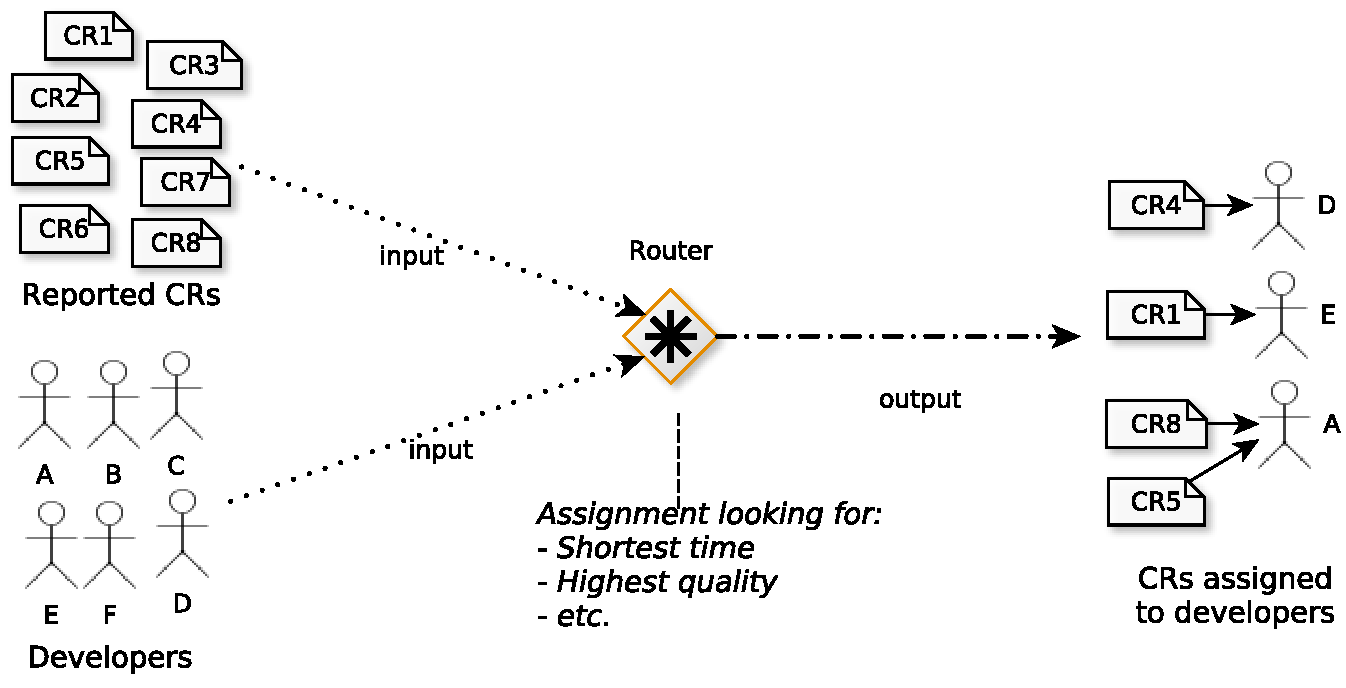
\includegraphics[width=\columnwidth]{images/assignment-schema.pdf}
  \caption[\ac{cr} assignment.]{\ac{cr} assignment. The router, which may be the
  \acs{ccb}, project leaders, or managers, must match \acp{cr} and developers in
  order to obtain the shortest fixing and highest quality.}
  \label{fig:assignment-schema}
\end{figure}

\lipsum[2-4]

Nevertheless, by increasing the amount of reported \acp{cr} or the size of the
development team, it is visible that the router becomes overloaded and the
\ac{cr} assignment becomes an intensive, error prone activity. It was confirmed
by \citet{Jeong2009}, which identified that 37\%-44\% of the \acp{cr} in Mozilla
and Eclipse projects did not reach the right developer in the first assignment.
These \acp{cr}, in turn, had their fixing time delayed because they needed to be
reassigned one or more times. Furthermore, if the \acp{cr} are not fixed by the
appropriate developers, there is also the chance of introducing new defects
during the \acp{cr} fixing.

In this context, we believe that it is necessary to develop methods and tools to
automate the assignment of \acp{cr} and ensure that the \acp{cr} are being
assigned to the appropriate developers. With these methods and tools, we could
reduce the time needed to perform the assignments and, given that the
appropriate developers are actually being selected, the quality and time for the
\ac{cr} fixing are also improved.

\section{Problem Statement}
\label{sec:intro-problem-statement}

As previously mentioned, software maintenance has been considered as the most
costly aspect of software development~\citep{swebok2004}. There is a myriad of
reasons for this situation. One of them is the many changes that are required
after software delivery due to poor documented and misunderstood requirements,
or simply because \emph{``the clients do not know what they
want''}~\citep{Brooks1995}.

Another reason is the fact that a set of development activities must be
inevitably performed in order to implement a change. For instance, for each
change to be implemented it is necessary to comprehend the existing software
artifacts, modify the software's source code to implement the change, perform
tests and verification, and deliver the new version of the software.
Additionally, very often, the implementation of the change ends up by
introducing new defects in the software.
   
A third reason is the management aspects of software maintenance. It is
necessary to keep track of all these changes that are performed, generally
considering different versions of the software and customers.

\lipsum[3-5]

\begin{enumerate}
  \item Firstly, the approaches available in the literature were designed to
  perform autonomously. That is, the software analysts do not have the control
  of the approach; they cannot modify the approach's behavior. Without
  such control, in turn, the approach cannot be properly calibrated. As a
  consequence, if the approach's performance is not satisfactory, it is simply
  discarded.
  \item Secondly, the reported values for accuracy of these approaches are
  still low. With low accuracy, the previous reason takes place. That is, as the
  approaches perform with low accuracy, and the software analysts do not have
  control over them, the approaches are simply discarded.
  \item Finally, the third reason concerns the lack of contextual information in
  those approaches. As is well known, software development companies are
  dynamic: developers move from projects; developers are hired/fired;
  developers enter in vacation or take a day off; and developers have different
  experiences. This dynamic influences the assignment of \acp{cr}. Thus,
  contextual information is a necessity in automated approaches.
\end{enumerate}

Based on this context, the main research question investigated by this thesis is:

\begin{description}
  \item[Research question] \emph{Is it possible to develop a new approach for
  automated \ac{cr} assignment with satisfactory accuracy, leveraging
  contextual information, and designed in order to put the software analysts in
  control of such approach?}
\end{description}

With the objective to answer this question, it is necessary to understand
current approaches available in the literature, choose the correct technologies
that could support dynamic environments and, mainly, understand the necessities
of software analysts regarding a new approach for automated \ac{cr} assignment.
Thus, the goal of the work described in this thesis can be stated as:

\begin{description}
  \item[Research objective] \emph{This work proposes an automated approach for
  \ac{cr} assignment which uses \ac{ir} models, expert systems, and
  context-aware information in order to select the appropriate developers. The
  approach is supported by the state-of-the-art in the management of \acp{cr} as
  well as by the understanding of the aspects concerning the \ac{cr} assignment
  activity itself.}
\end{description} 

\section{Overview of the Proposal}
\lipsum[1-5]

\section{Research Methodology}

This research design of this thesis is based on a multimethod
approach~\citep{Hesse-Biber2010}. Such approach combines two or more
quantitative (or qualitative) methods in a single study, such as a survey and an
experiment~\citep{Hesse-Biber2010}. Multimethod must not be confused with mixed
method. In this last, methods for both qualitative and quantitative types of
research are applied in a single study. On the other hand, multimethod studies
combine different methods for a single research type.

When applying a multimethod approach, the triangulation is used to consolidate
the results from the different methods, considering, however, that the same
research question(s) was/were investigated in these methods. As a consequence,
the triangulation of methods enhances the conclusions and completeness of the
study, bringing more credibility to the research
findings~\citep{Hesse-Biber2010}. \figref{fig:research-methodology-thesis} shows
the multimethod research design applied in this thesis.

\begin{figure}[h]
\centering
  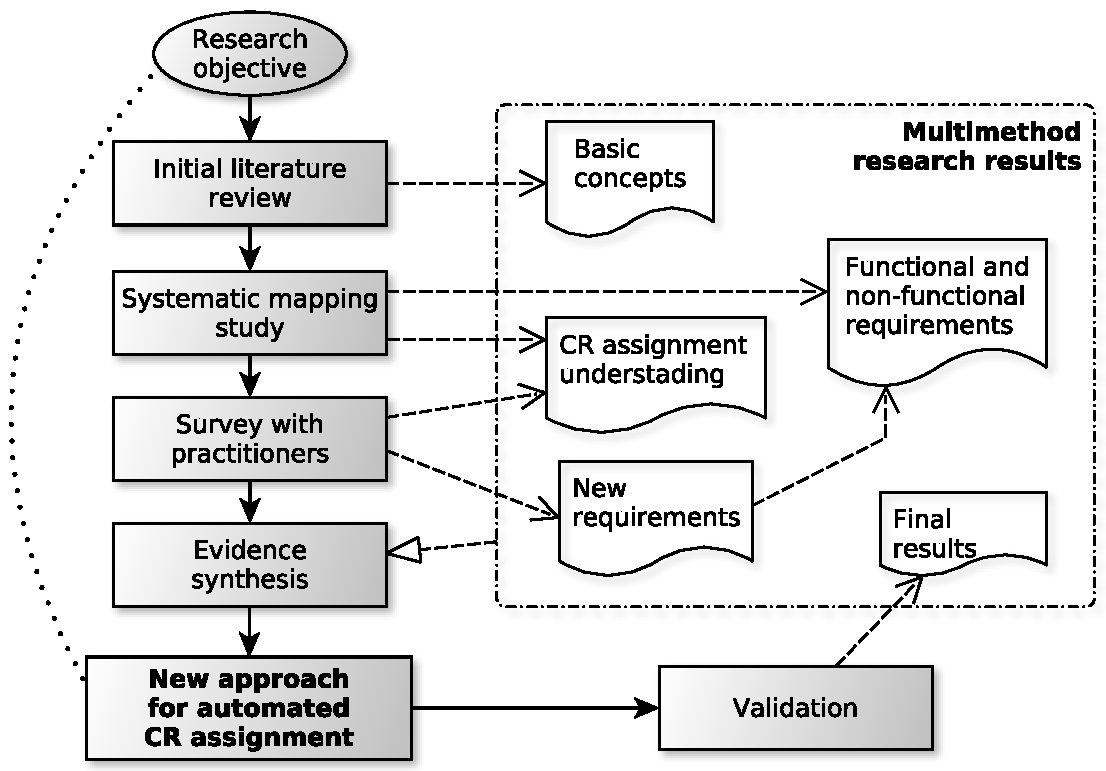
\includegraphics[width=\columnwidth]{images/research-methodology-thesis.pdf}
  \caption[Research methodology.]{The research methodology applied for this
  thesis.}
  \label{fig:research-methodology-thesis}
\end{figure}

The design started by stating the research objective, which we defined in
\secref{sec:intro-problem-statement}, and performing the initial literature
review. This last provided the basic concepts and understanding of the area.
Then, a systematic mapping study and a questionnaire-based survey were
conducted. These two gathered detailed information on our research topic.
Indeed, both of them were used to understand the key aspects of \ac{cr}
assignment and identify the set of requirements to automate the assignments. In
the evidence synthesis step, these results were detailed and organized in order
to formulate the approach to automate \ac{cr} assignments, which was constructed
in the next step. Finally, the research design states the validation of the
proposed approach.

\section{Out of Scope}

As the proposed approach is part of a broader context, a set of related aspects
will be left out of its scope. Thus, the following topics are not directly
addressed in this thesis:

\begin{enumerate}
  \item \textbf{Tools for \ac{cr} management.} We are addressing
  a specific aspect of \ac{cr} management, which is the \ac{cr} assignment
  activity. Thus, it is out of scope of this thesis to provide a
  complete solution for \ac{cr} management. Instead, we are planning to
  implement standalone software which will be able to integrate with the
  most well known tools for \ac{cr} management, such as Mantis, Bugzilla, and
  Trac, providing a service to leverage the automation of \ac{cr}
  assignments.
  
  \item \textbf{Software maintenance process.} Software maintenance involves
  a set of activities aiming at implementing modifications in some software
  project. These activities must be coordinated through a process so that the
  maintenance can be successful. In Chapter 2, we discuss some of
  these processes. However, in this thesis, we are not concerned with the
  maintenance process itself. Actually, it should be transparent in our approach
  to automate \ac{cr} assignment. Thus, it is out of scope of this
  thesis to provide any process assessment for software maintenance beyond the
  activity of \ac{cr} assignment.
  
  \item \textbf{\ac{ir} models.} Many models for \ac{ir} have been proposed for
  different objectives, including the \ac{cr} assignment itself. However, due to
  the broad availability of these models, it is out of scope of this thesis to
  develop a new one. Instead, the \ac{ir} models with better performance,
  identified through the systematic mapping study, were chose to be
  integrated in our approach;
  
  \item \textbf{Rule-based expert systems.} Similar to \ac{ir} models,
  rule-based expert systems have a long history of development. Thus, our
  approach does not intend to develop a whole new system with this purpose.
  Actually, we integrated in our approach the
  Drools\footnote{\url{http://www.jboss.org/drools/}} expert system, which is a
  mature tool that can be easily manipulated;
  
  \item \textbf{Mathematical formulations on NP-Complete problems.} We
  understand that the problem of assigning \acp{cr} to software developers is in
  the broad category of \emph{assignment problems}, which is well known to be
  NP-Complete. Thus, could be formulated as such. However, the mathematical
  formulations of the \ac{cr} assignment problem is out of scope of this thesis.
  As well as finding an optimal solution on the context of NP-Complete problems
  is also out of scope. The main reason for this is the human factors and
  context variables that are involved in the assignment of \acp{cr}, which
  make this problem hard to be computable. A mathematical formulation of the
  \ac{cr} assignment problem is provided by~\citet{Rahman2009}.
\end{enumerate}

\section{Statement of the Contributions}
\lipsum[6-7]

\begin{enumerate}
  \item An overview of the software maintenance concepts and processes, with
  emphasis on the importance of \ac{cr} management aspects; 
  \item A survey performed with practitioners from a large organization, in
  order to understand the aspects of the \ac{cr} assignment
  activity. Published in the \emph{17$^{th}$ International Conference on Evaluation
  and Assessment in Software Engineering (EASE'2013)}~\citep{CavalcantiEASE2013};
  \item A replication of the previous survey in two more organizations;
  \item A systematic mapping study performed to understand the challenges and
  opportunities of \ac{cr} management, as well as to identify research gaps and
  the road ahead. Accepted for publication in the
  \emph{Journal of Software: Evolution and Process}~\citep{CavalcantiJSEP2013};
  \item The definition of the functional and non-functional requirements that
  are required to effectively automate \ac{cr} assignment, which takes as input
  the systematic mapping study and the survey;
  \item The definition of an approach that satisfies the
  identified requirements to automate the \ac{cr} assignment activity;
  \item The realization of the proposed approach's architecture, in which we
  described the methods and techniques used for the implementation, as well as the
  components that have to be built and the third party components that should be
  assembled together in order to provide a service for automated \ac{cr}
  assignment; and
  \item The evaluation of the proposed approach, performed as an offline
  experiment simulating a real context.
\end{enumerate}

\section{Organization of the Thesis}

\lipsum[5-10]
\chapter{Background Chapter}

\section{Introduction}

\lipsum[1-4]

\section{Section}

\lipsum[2-4]

\subsection{Subsection}

\lipsum[2-4]
\chapter{Development Chapter}

\section{Introduction}

\lipsum[1-4]

\section{Section}

\lipsum[2-4]

\subsection{Subsection}

\lipsum[2-4]
\chapter{Conclusion}

\section{Introduction}

\lipsum[1-4]

\section{Section}

\lipsum[2-4]

\subsection{Subsection}

\lipsum[2-4]

% References

\begin{references}
  \bibliography{references}
\end{references}

% Appendix

\theappendix
\chapter{Mapping Study's Instruments}
\label{ap:mapping-study}

\begin{table}[!htp]
	\centering
	\caption{List of conferences on which the searches were performed.}
	\label{tbl:conferences_list}
	\rowcolors{2}{lightgray!30}{white}
	\resizebox{\columnwidth}{!}{
	\begin{tabular}{ll}
	\toprule
	\textbf{Acronym} & \textbf{Conference} \\
	\toprule
	APSEC & Asia Pacific Software Engineering Conference \\
	ASE   & IEEE/ACM International Conference on Automated Software Engineering \\
	CSMR  & European Conference on Software Maintenance and Reengineering \\
	ESEC  & European Software Engineering Conference \\
	ESEM  & International Symposium on Empirical Software Management and Measurement \\
	ICSE  & International Conference on Software Engineering \\
	ICSM  & International Conference on Software Maintenance \\
	ICST & International Conference on Software Testing \\
	InfoVis & IEEE Information Visualization Conference \\
	KDD   & ACM SIGKDD International Conference on Knowledge Discovery and Data Mining \\
	MSR   & Working Conference on Mining Software Repositories \\
	OOPSLA & Object-Oriented Programming, Systems, Languages and Applications \\
	QSIC  & International Conference On Quality Software \\
	SAC & ACM Symposium on Applied Computing \\
	SEAA & EUROMICRO Conference on Software Engineering and Advanced Applications\\
	SEDE & 19th International Conference on Software Engineering and Data Engineering \\
	SEKE  & International Conference on Software Engineering and Knowledge Engineering \\
	\bottomrule
	\end{tabular}
	}
\end{table}

\begin{table}[htp]
	\caption{List of journals in which the searches were performed.}
	\label{tbl:journals_list}
	\centering
	\rowcolors{2}{lightgray!30}{white}
	\begin{tabular}{l}
	\toprule
	\textbf{Journal title} \\
	\toprule
	ACM Transactions on Software Engineering and Methodology \\
	Automated Software Engineering \\
	Elsevier Information and Software Technology \\
	Elsevier Journal of Systems and Software \\
	Empirical Software Engineering \\
	IEEE Software \\
	IEEE Computer \\
	IEEE Transactions on Software Engineering \\
	International Journal of Software Engineering and Knowledge Engineering \\
	Journal of Software: Evolution and Process \\
	Software Quality Journal \\
	Journal of Software \\
	Software Practice and Experience Journal \\
	\bottomrule
	\end{tabular}
\end{table}

\begin{table}[h]
\centering
\footnotesize
 \rowcolors{2}{lightgray!30}{white}
\caption{Search string per Search Engine.}
\label{tbl:stringengine}
\begin{tabular}{p{.15\textwidth}p{.8\textwidth}}
\toprule
\textbf{Search Engine} & \textbf{Search String}\\
\toprule
   	 	Google Scholar &  bug report OR track OR triage ``change
   	 	request'' issue track OR request OR software OR ``modification request'' OR
   	 	``defect track'' OR ``software issue''  repositories maintenance evolution\\

   	 	ACM Portal & Abstract: "bug report" or Abstract:"change request"
   	 	or Abstract:"bug track" or Abstract:"issue track" or  Abstract:"defect
   	 	track" or Abstract:"bug triage" or Abstract: "software issue" or Abstract: "issue request"
   	 	or Abstract: "modification request") and  (Abstract:software or
   	 	Abstract:maintenance or Abstract:repositories or Abstract:repository \\

   	 	IEEExplorer (1) & (((((((((("Abstract": "bug report") OR
   	 	"Abstract":"change request") OR "Abstract":"bug track") OR "Abstract":"software issue") OR "Abstract":"issue request") OR
        "Abstract":"modification request") OR "Abstract":"issue track") OR
	    "Abstract":"defect track") OR "Abstract":"bug triage") AND
	    "Abstract":software)\\

         IEEExplorer (2) & (((((((((("Abstract": "bug report") OR
         "Abstract":"change request") OR "Abstract":"bug track") OR "Abstract":"software issue") OR
         "Abstract":"issue request") OR "Abstract":"modification request") OR
         "Abstract":"issue track") OR "Abstract":"defect track") OR
         "Abstract":"bug triage") AND "Abstract":maintenance)\\

         IEEExplorer (3) & (((((((((("Abstract": "bug report") OR
         "Abstract":"change request") OR "Abstract":"bug track") OR "Abstract":"software issue") OR
         "Abstract":"issue request") OR "Abstract":"modification request") OR
         "Abstract":"issue track") OR "Abstract":"defect track") OR
         "Abstract":"bug triage") AND "Abstract":repositories)\\

         IEEExplorer & (((((((((("Abstract": "bug report") OR
         "Abstract":"change request") OR "Abstract":"bug track") OR "Abstract":"software issue") OR
         "Abstract":"issue request") OR "Abstract":"modification request") OR
         "Abstract":"issue track") OR "Abstract":"defect track") OR
         "Abstract":"bug triage") AND "Abstract": repository)\\

         Citeseer Library & (abstract: "bug report" OR abstract:"change request" OR abstract:"bug track" OR abstract:"issue track" OR
	     abstract:"defect track" OR abstract:"bug triage" OR abstract: "software
	     issue" OR abstract: "issue request" OR abstract: "modification request")
	     AND (abstract:software OR abstract:maintenance OR abstract:repositories OR
	     abstract:repository)\\

	     Elsevier & ("bug report" OR "change
	     request" OR "bug track" OR "issue track" OR "defect track" OR "bug triage" OR "software issue" OR  "issue request" OR
	    "modification request") AND (software OR maintenance OR repositories OR
	    repository)\\

	    Scirus & ("bug report" OR "change request" OR "bug track" OR "issue track" OR  "defect track" OR "bug triage" OR
        "software issue" OR  "issue request" OR "modification request") AND
	    (software maintenance OR repositories OR repository) ANDNOT (medical OR
	    aerospace)\\

	    ScienceDirect & ("bug report" OR "change request" OR "bug track"
	     OR "issue track" OR "defect track" OR "bug triage" OR "issue request" OR
	     "modification request") AND LIMIT-TO(topics, "soft ware")\\

	     Scopus & ("bug report" OR "change request" OR "bug track" OR
	     "issue track" OR  "defect track" OR "bug triage" OR "software issue" OR
	     "issue request" OR "modification request") AND (software maintenance OR
	     repositories OR repository)\\

	     Wiley & ("bug report" OR "change request"
	     OR "bug track" OR "issue track" OR  "defect track" OR "bug triage" OR
         "software issue" OR  "issue request" OR "modification request") AND
	     (software maintenance OR repositories OR repository)\\

	     ISI Web\newline of Knowledge & ("bug report" OR "change request" OR "bug
	     track" OR "issue track" OR  "defect track" OR "bug triage" OR "software issue" OR  "issue request" OR "modification request") AND
	    (software maintenance OR repositories OR repository) ANDNOT (medical OR
	    aerospace)\\

	    SpringerLink & ("bug report" OR "change request" OR "bug track" OR "issue track" OR  "defect track" OR "bug triage" OR
        "software issue" OR  "issue request" OR "modification request") AND
	    (software maintenance OR repositories OR repository) ANDNOT (medical OR
	    aerospace)\\
	\bottomrule
\end{tabular}
\end{table}

\end{document}
